\section{Bewertung der Daten in Grafana}

%Mit dieser Arbeit wollten wir eine \gls{opensource} ähnliche \gls{SIEM} Lösung verwenden, um Überwachungsmechanismen über Logdateien zu erstellen. Die folgende Tabelle vergleicht die existierenden Funktionalitäten eines \gls{SIEM} mit denen, die wir mit unserem Aufbau erreichten:

In dieser Arbeit haben wir versucht, eine \gls{opensource}-basierte Lösung ähnlich einem \gls{SIEM} zu verwenden, um Überwachungsmechanismen anhand von Logdateien zu erstellen. In der folgenden Tabelle vergleichen wir die vorhandenen Funktionalitäten eines \gls{SIEM} mit denen, die wir durch unsere Implementierung erreichen konnten.

\begin{table}[H]
    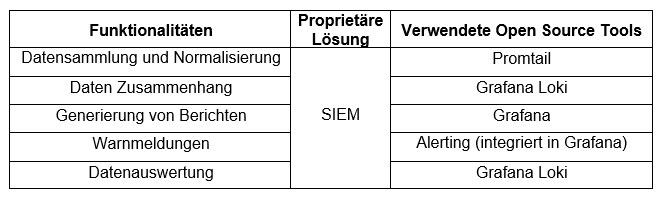
\includegraphics[width=\linewidth]{assets/tabelle_siem_BA.png}
    \caption{Verwendete Tools für den Aufbau einer \gls{SIEM} ähnlichen Lösung\\Quelle: Eigene Quelle und \citep{Granadillo_SIEM}}
 \end{table}
 
%Aus einer prinzipiellen Sicht können wir behaupten, dass die verwendeten Tools eine kostengünstige Möglichkeit anbieten, eine Überwachungssystem in einem Rechenzentrum zu implementieren. Die Methoden für Angriffserkennung lassen sich von der \gls{mitre} Matrix oder von anderen Framework deutlich definieren. Nach der Auswhal des Angriffes, erstellen wir Regelsätze mit der Abfragesprache \gls{logql} in Loki, um Muster zu identifieren, die auf den ausgewählten Angriff hindeuten. Wir benutzen dann diese Regelsätze, um Warnmeldung über den Angriff zu generieren und zu schicken.

Aus prinzipieller Sicht können wir feststellen, dass die verwendeten Tools eine kosteneffektive Möglichkeit bieten, ein Überwachungssystem in einem Rechenzentrum zu implementieren. Die Methoden zur Erkennung von Angriffen lassen sich klar anhand der \gls{mitre}-Matrix oder anderer Frameworks definieren. Nach der Auswahl des Angriffs erstellen wir Regelwerke mit der Abfragesprache \gls{logql} in Loki, um Muster zu identifizieren, die auf den ausgewählten Angriff hindeuten. Diese Regelwerke werden dann verwendet, um Warnmeldungen über den Angriff zu generieren und zu versenden.

%Unser Aufbau hat zwei große Herausforderungen. Die erste lässt sich einfacher beseitigen als die zweite. Diese sind:

Unser Aufbau birgt zwei große Herausforderungen, wobei die erste einfacher zu bewältigen ist als die zweite. Diese sind:

\begin{itemize}[noitemsep]
    \item \textbf{Definition der Regelsätzen}
\end{itemize}

%Für eine präzise Implementierung spielt die richtige Entwicklung der Regelsätzen für die Identifizierung des potenziellen Angriffes eine wesentliche Rolle. Da Logdateien aus produktiven Umgebungen große Menge von Information beinhalten, müssen diese Regelsätze so festgelegt werden, dass sie die eindeutige Informationen, wie IP-Adresse, Portnummer, Zeitfenster und Abstandzeit zwischen Anfrage, filtern und nach Angriffsmuster kategorisieren.

Für eine präzise Implementierung spielt die richtige Entwicklung der Regelsätzen zur Identifizierung potenzieller Angriffe eine wesentliche Rolle. Da Logdateien aus produktiven Umgebungen eine große Menge an Informationen enthalten, müssen diese Regelsätzen so definiert werden, dass sie die eindeutigen Informationen wie IP-Adresse, Portnummer, Zeitfenster und Zeitabstände zwischen Anfragen filtern und nach Angriffsmustern kategorisieren können.

\begin{itemize}[noitemsep]
    \item \textbf{statische Regel in einer dynamischen Angriffswelt}
\end{itemize}

Die von uns definierten Regeln haben statische Elemente wie die \quotes{Anzahl von Anfragen}, den \quotes{Zeitabstand zwischen Requests} und die \quotes{Anzahl von fehlgeschlagenen Anmeldeversuchen}. Die heutigen Angriffe haben jedoch auch einen dynamischen Aspekt, der sich an die Umgebung anpasst, insbesondere durch die starke Entwicklung von \glsfirst{KI}. Während \gls{KI} einerseits für die Automatisierung von Aufgaben oder für effiziente Datenanalyse verwendet wird, könnte sie auch für Cyberkriminalität genutzt werden. \gls{KI} ist am Ende nur ein Werkzeug, dessen Nutzung von den Absichten ihrer Benutzer abhängt.

%Die von uns definierten Regel haben statische Elementen, wie \quotes{Anzahl von Anfrage}, \quotes{Zeitabstand zwischen Requests}, \quotes{Anzahl von fehlgeschlagenen Anmeldeversuchen}. Die heutigen Angriffe haben aber einen dynamischen Aspekt, die sich an der Umgebung anpasst, besonders mit der starken Entwicklung von \glsfirst{KI}. Während \gls{KI} einerseits für Automatisierung von Aufgabe oder für effiziente Datenanalyse verwendet wird, könnte sie auch für Cyberkriminalität zur Nutzung kommen. \gls{KI} ist am Ende nur ein Tool, dessen Nutzung von den Absichten ihrer Benutzer abhängig ist.

Verschiedene Angriffstechniken lassen sich schneller und effizienter mit \gls{KI} durchführen. Die Nutzung von \gls{polyphomicMalware} ist ein Beispiel, wo weder Antivirus-Programme noch Log-Analyse-Tools einen normalen von einem abnormalen Ablauf unterscheiden können. Auch die Verkehrsanalyse kann durch \gls{KI} gefährdet sein, da Angriffe und normaler Verkehr ähnlich dargestellt werden können. Darüber hinaus kann \gls{KI} auch gegen Authentifizierungsverfahren eingesetzt werden, um beispielsweise Anmeldedaten schneller zu erraten und/oder vorauszusehen \citep{Fritsch_AIcybersec}.


%Verschiedenen Angriffstechniken lassen sich schneller und effizienter mit \gls{KI} durchführen. Die Nutzung von \gls{polyphomicMalware} ist ein Beispiel, wo weder Antivirus-Programmen noch Log-Analyse-Tools einen normalen von abnormalen Ablauf unterscheiden können. Die Verkehrsanalyse können auch durch \gls{KI} gefährdet sein, da Angriffe und normaler Verkehr sich ähnlich darstellen lassen. Und auch gegen Authentifizierungsverfahren kann \gls{KI} verwendet werden, um z.B.Anmeldedaten schneller zu raten und/oder vorauszusehen \citep{Fritsch_AIcybersec}. 

\newpage
Das folgende Diagramm zeigt, wo sich \gls{KI} bei Cyberangriffen anhand der\gls{CKC} integrieren lässt:

%Das folgende Diagramm stellt dar, wo sich \gls{KI} bei Cyberangriffen anhand der \gls{CKC} integrieren lässt:

\begin{figure}[H]
    \centering
    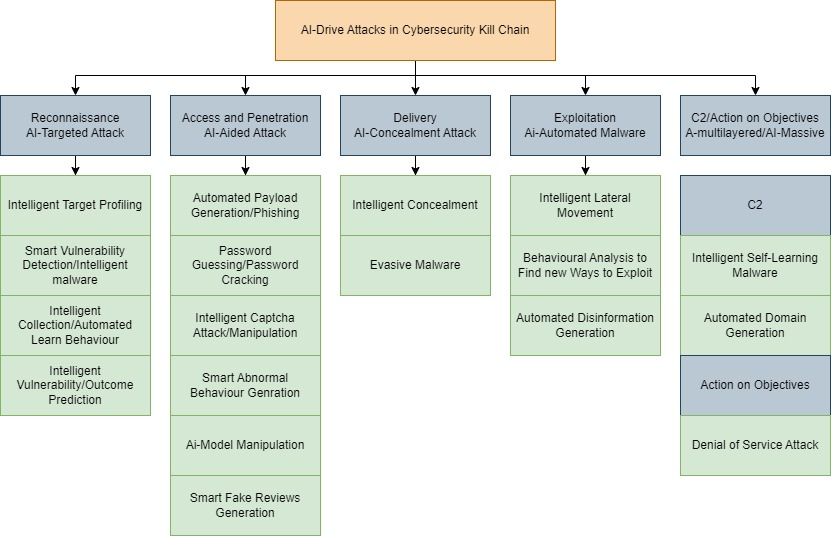
\includegraphics[width=0.9\textwidth]{assets//CKC_AI.jpg}
    \caption{\gls{KI} in der \glsfirst{CKC} \\Quelle: \citep{Guembe_AIDiagrammAngriff}}
    \centering
 \end{figure}
 
\subsection{Zukünftige Entwicklungen}
Um sicherzustellen, dass unsere vorgeschlagenen Lösungen sich an diese neue und dynamische Realität anpassen können, können zukünftige Regelsätze mithilfe von \gls{KI} erstellt werden. Nachdem die meisten möglichen Angriffsflächen abgedeckt wurden, sollten die Regeln so angepasst werden, dass sie möglichst viele Szenarien abdecken.

%Damit unsere vorgeschlagenen Lösung sich an diese neue und dynamische Realität anpasst, können zukünftige Regelsätze mithilfe von \gls{KI} aufgebaut werden. Nachdem die meisten möglichen Angriffsoberfläche gedeckt wurden, sollen die Regel so angepasst werden, dass sie verschiedenen viele Szenarien decken.

Mit der rasanten Entwicklung von \gls{KI}, insbesondere während der Erstellung dieser Arbeit, können wir auch erwarten, dass sich sowohl Loki als auch Grafana bald mit verschiedenen \gls{opensource} \gls{plugin} integrieren lassen, die auch \gls{KI} unterstützen, um die Loganalyse effizienter und zuverlässiger zu machen. All dies würde dazu beitragen, einen sicheren Netzwerkverkehr zu gewährleisten.


